\documentclass[sigplan,10pt,anonymous,review]{acmart}\settopmatter{printfolios=true,printccs=false,printacmref=false}

\usepackage{tikz}
\usetikzlibrary{arrows}
\usepackage{proof}

\newcommand{\ra}{\rightarrow}
\newcommand{\Ra}{\Rightarrow}
\newcommand{\Set}{\mathsf{Set}}
\newcommand{\Prop}{\mathsf{Prop}}
\newcommand{\Ty}{\mathsf{Ty}}
\newcommand{\Tm}{\mathsf{Tm}}
\newcommand{\Con}{\mathsf{Con}}
\newcommand{\Sub}{\mathsf{Sub}}
\newcommand{\Tel}{\mathsf{Tel}}
\newcommand{\Tms}{\mathsf{Tms}}
\newcommand{\p}{\mathsf{p}}
\newcommand{\q}{\mathsf{q}}
\newcommand{\ext}{\mathop{\triangleright}}
\newcommand{\N}{\mathbb{N}}
\newcommand{\lam}{\mathsf{lam}}
\newcommand{\app}{\mathsf{app}}
\newcommand{\U}{\mathsf{U}}
\newcommand{\El}{\mathsf{El}}
\newcommand{\cd}{\mathsf{c}}
\newcommand{\blank}{\mathord{\hspace{1pt}\text{--}\hspace{1pt}}} %from the book
\renewcommand{\tt}{\mathsf{tt}}
\newcommand{\fst}{\mathsf{fst}}
\newcommand{\snd}{\mathsf{snd}}
\newcommand{\Lift}{\mathsf{Lift}}
\newcommand{\mk}{\mathsf{mk}}
\newcommand{\un}{\mathsf{un}}
\newcommand{\id}{\mathsf{id}}

\begin{document}

\newtheorem{problem}[theorem]{Problem}
\theoremstyle{remark}
\newtheorem{construction}[theorem]{Construction}

\title{Type theory in type theory with single substitutions}
\author{Ambrus Kaposi and Szumi Xie}
\date{\today}

\begin{abstract}
Type theory can be described as a generalised algebraic theory. This
automatically gives a notion of model and the existence of the syntax
as the initial model, which is a quotient inductive-inductive
type. Algebraic definitions of type theory include Ehrhard's
definition of model, categories with families (CwFs), contextual
categories, Awodey's natural models, C-systems, B-systems. With the
exception of B-systems, these notions are based on a parallel
substitution calculus where substitutions form a category. In this
paper we define a single substitution calculus (SSC) for type theory
and show that the SSC syntax and the CwF syntax are isomorphic for a
theory with dependent function space and a hierarchy of universes. SSC
only includes single substitutions and single weakenings, and eight
equations relating these: four equations describe how to substitute
variables, and there are four equations on types which are needed to
typecheck other equations. All the other equations are substitution
(naturality) rules or computation rules for different type
formers. SSC provides a simple, minimalistic alternative to parallel
substitution calculi or B-systems for defining type theory. SSC
relates to CwF as extensional combinatory calculus relates to lambda
calculus. All the results in this paper were formalised in Agda.
\end{abstract}

\maketitle

\section{Introduction}

What is type theory? Here we refer to type theory as a particular
formal system based on Martin-Löf's original definition
\cite{martinlof73predicative}, and not to the study of type systems
(e.g.\ \cite{DBLP:books/daglib/0005958}).

Type theory is a language which can be described as a second-order
generalised algebraic theory (SOGAT
\cite{DBLP:conf/fscd/KaposiX24}). Some properties of this description:
\begin{enumerate}
\item[(i)] It is an intrinsic presentation
  \cite{DBLP:conf/csl/AltenkirchR99,DBLP:conf/popl/AltenkirchK16} as
  opposed to extrinsic \cite{abel2013normalization,theo}. That is, we
  only consider well-formed, well-scoped and well-typed abstract
  syntax trees, there are no meaningless terms.
\item[(ii)] Terms are quotiented by the conversion relation.
\item[(iii)] Every operation is stable under substitution.
\end{enumerate}
For example, type theory with $\Pi$ types and universes {\`a} la
Coquand \cite{coquandUniverse} is specified by the following SOGAT.
\begin{equation}\label{eq:tt}
\begin{alignedat}{10}
  & \Ty && : \N\ra\Set \\
  & \Tm && : \Ty\,i\ra\Set \\
  & \Pi && : (A:\Ty\,i)\ra(\Tm\,A\ra\Ty\,i)\ra\Ty\,i \\
  & \app && : \Tm\,(\Pi\,A\,B)\cong((a:\Tm\,A)\ra\,\Tm\,(B\,a)): \lam \\
  & \U && : (i:\N)\ra\Ty\,(1+i) \\
  & \El && : \Tm\,(\U\,i)\cong\Ty\,i : \cd \\
  & \Lift && : \Ty\,i\ra\Ty\,(1+i) \\
  & \un && : \Tm\,(\Lift\,A)\cong\Tm\,A : \mk
\end{alignedat}
\end{equation}
Because types are isomorphic to a term (witnessed by $\El$ and $\cd$),
we have to index types by their (universe) level, and types at lower
levels are included at upper levels by $\Lift$. We use implicit
arguments, e.g.\ $\Tm$ takes the $i:\N$ implicitly, and $\app$ takes
$i$, $A$ and $B$ implicitly. $f : X \cong Y : g$ denotes an
isomorphism, that is, $f : X\ra Y$, $g:Y\ra X$ with $g\,(f\,x) = x$
and $f\,(g\,y) = y$ for all $x$, $y$. Note that $\Pi$ and $\lam$ are
second-order functions. We say that $\Pi$ binds a $\Tm$-variable of
type $A$ in its second $\Ty$-argument. Every binder is represented by
a second-order function, and as a result, we don't need to talk about
contexts and substitutions when describing the theory: we re-use the
binding features of the metatheory to describe those of our object
theory (this technique is also known as higher-order abstract syntax
\cite{DBLP:conf/lics/Hofmann99} or logical framework
\cite{DBLP:journals/jacm/HarperHP93,10.1007/978-3-642-14203-1_2} and
our notation comes from two-level type theory \cite{DBLP:conf/csl/AltenkirchCK16,DBLP:journals/mscs/AnnenkovCKS23}). There is no good notion of homomorphism between
second-order models, thus the semantics of a SOGAT is given by a first
order generalised algebraic theory (GAT
\cite{DBLP:journals/apal/Cartmell86}). GATs are generalisations of
single-sorted algebraic theories (such as monoids, groups) to multiple
sorts where later sorts can be indexed over previous sorts. The usual
results from universal algebra (e.g.\ models form a category with
finite limits and initial object, existence of free and co-free
models) carry over to GATs \cite{andras,DBLP:phd/hal/Moeneclaey22}. An
example of a GAT is the theory of categories where there is a sort of
objects and a sort of morphisms double-indexed over objects.

Kaposi and Xie \cite{DBLP:conf/fscd/KaposiX24} present two different
first order semantics for any SOGAT: one based on parallel
substitutions, and one based on single substitutions.

In the parallel semantics, the GAT always starts with a category with
a terminal object, objects of the category are called contexts,
morphisms are substitutions. Every sort/operation of the SOGAT gives
rise to a sort/operation in the GAT which is now indexed by
contexts. The sorts moreoever come with instantiation (sometimes
called substitution) operations which are functorial, and all the
operations are natural with respect to instantiation. For those sorts
which are bound by an operation in the SOGAT description, we have
context extension, meaning that contexts can carry variables of that
sort (in other words, the sort is given by a locally representable
presheaf). The parallel semantics of the SOGAT
\begin{equation}\label{eq:tytm}
\begin{alignedat}{10}
  & \Ty && : \Set \\
  & \Tm && : \Ty \ra\Set 
\end{alignedat}
\end{equation}
is the GAT of categories with families (CwFs
\cite{DBLP:conf/types/Dybjer95,Castellan2021}, Definition \ref{def:cwf}).
We define the notion ``model of the SOGAT'' by its parallel substitution
semantics, which is a GAT, and that has an obvious notion of model. The
syntax of the language is the initial model, which exists for every
GAT \cite{DBLP:journals/pacmpl/KaposiKA19}. This is an intrinsic
syntax (only well-typed terms), quotiented by the equations in the
SOGAT, which describe conversion for the language.

The single substitution semantics is a GAT which does not start with a
category: there are contexts and maps between contexts, but these maps
are single substitutions or single weakenings, they don't
compose. There are fewer operations and fewer equations than in the
parallel semantics. In this paper we investigate the single
substitution semantics of the type theory specified by the SOGAT
(\ref{eq:tt}). This presentation of type theory is simpler than CwFs,
the operations are all easy to motivate, we illustrate this in Section
\ref{sec:tt}. Single substitution calculi are closer to the usual
presentation of type theory using derivation rules, this was one of
the motivations of Voevodsky for developing B-systems
\cite{AHRENS_EMMENEGGER_NORTH_RIJKE_2023}. Our single substitution
semantics of (\ref{eq:tytm}) is simpler and has more models than
B-systems. GAT presentations of type theory are important for defining
models. Our presentation gives a new notion of model, which in the
future might contribute to definitions of new models. It can also
influence implementations of type theory. Because our single
substitution GAT does not involve a category, it might be easier to
adapt it to a higher dimensional setting, see Section
\ref{sec:conclusion}.

The single substitution semantics is in some sense
too minimalistic: for example, consider a term $b$ which depends on a
context $\Gamma$ and an extra variable of type $A$, that is, $b :
\Tm\,(\Gamma\ext A)\,B$. We weaken $b$ so that we add an extra $A$
variable \emph{before} the last one obtaining $ b[\p^+] :
\Tm\,(\Gamma\ext A\ext A[\p])\,(B[\p]) $ where $\p$ is weakening at
the end of the context, and $\p^+$ is weakening just before the last
variable in the context. Then, we instantiate the last $A[\p]$
variable in the context by the previous $A$ obtaining
$b[\p^+][\langle\q\rangle] : \Tm\,(\Gamma\ext A)\,B$ where $\q$
denotes the last variable in the context (a.k.a\ De Bruijn index $0$).
We cannot derive $b[\p^+][\langle\q\rangle] = b$ in an arbitrary single substitution
model, but this equation holds in the single substitution syntax.
% p⁺  : Sub (Γ▹A▹A[p]) (Γ▹A)
% ⟨q⟩ : Sub (Γ▹A) (Γ▹A▹A[p])
This is analogous to e.g.\ parametricity results
\cite{DBLP:journals/jfp/BernardyJP12}, which do not hold in an
arbitrary model, but they hold in the syntax. In fact, we show that
the single substitution syntax of (\ref{eq:tt}) is equivalent to the
parallel substitution syntax of (\ref{eq:tt}), and the techniques that
we use are not specific to the SOGAT (\ref{eq:tt}), we expect
that they work for any SOGAT. Equivalence of the syntaxes means that
the corresponding sorts ($\Con$, $\Ty$, $\Tm$) are isomorphic. For a
general SOGAT, there are more models of the correponding single
substitution GAT than the parallel substitution GAT. Every parallel
model is also a single model, but not necessarily the other way. While
B-systems are equivalent to CwFs (and C-systems
\cite{AHRENS_EMMENEGGER_NORTH_RIJKE_2023}), there are more single
substitution models of (\ref{eq:tytm}) than parallel substitution
models. The situation is similar to that of extensional combinatory
calculus and lambda calculus, where the syntaxes are equivalent, and
every lambda model is a combinatory model, but not the other way round
\cite{DBLP:conf/fscd/AltenkirchKSV23}. A simpler example is the
relationship of monoids over a set $X$ and nil/cons algebras over $X$,
where every monoid is a nil/cons-algebra, but not the other way; it is
well-known that free monoids over $X$ (syntax for monoid over $X$) are
the same as lists of $X$ (the syntax for nil/cons algebras over $X$).

When showing that the parallel and single substitution syntaxes are
equivalent, we define the parallel operations by induction on the
single substitution syntax. One of the operations in the single
substitution syntax is the instantiation operation: $\blank[\blank] :
\Ty\,\Gamma\ra\Sub\,\Delta\,\Gamma\ra\Ty\,\Delta$, and similarly for
terms. When doing induction on types/terms, we have to provide
a method for these operations, but this can be difficult as
substitutions don't compose. This is why we derive a new induction
principle which works on $\alpha$-normal types and terms. Just as
$\beta$-normal forms don't distinguish between $\beta$-equal terms,
$\alpha$-normal forms don't include explicit substitutions.
$\alpha$-normal forms are not usual normal
forms in the sense that they are still quotiented by the
computation/uniqueness rules like $\beta$/$\eta$ for function
space. To derive the new induction principle for the syntax, we first
prove $\alpha$-normalisation.

In the particular theory (\ref{eq:tt}), every type is represented by a
term. In its single substitution calculus, this can be
used to adapt some equations and remove some others, obtaining a more
minimalistic, but equivalent GAT.

Theory (\ref{eq:tt}) can be extended
with unit and $\Sigma$ types, more precisely with the following rules.
\begin{equation}\label{eq:sigma}
  \begin{alignedat}{10}
    & \top && : \Ty\,0 \\
    & \tt && : \Tm\,\top \\
    & \top\eta && : t = \tt \\
    & \Sigma && : (A:\Ty\,i)\ra(\Tm\,A\ra\Ty\,i)\ra\Ty\,i \\
    & \fst,\snd && : \Tm\,(\Sigma\,A\,B)\cong(a:\Tm\,A)\times\,\Tm\,(B\,a): \blank,\blank
\end{alignedat}
\end{equation}
Using the same insight about types and the universe, the fact that
dependences can be represented by function spaces, and that
collections of dependencies can be collected using $\Sigma$ types, we
can actually derive a parallel model from any single substitution
model. This way we show that for the particular theory (\ref{eq:tt})+(\ref{eq:sigma}),
single and parallel substitution models are actually equivalent in a
weak sense.

To summarise, our contributions are the following:
\begin{itemize}
\item A new generalised algebraic presentation of type theory in the
  form of a minimalistic single substitution calculus. We show that
  there is no need for parallel substitutions, empty substitution,
  parallel weakenings, telescopes, or combinations of these to
  describe the syntax of type theory in an intrinsic way.
\item The $\alpha$-normalisation technique and deriving parallel
  substitutions from the single substitution syntax.
\item For type theory with $\Pi$, $\U$, a minimised presentation of
  the equations which results in an isomorphic theory.
\item For type theory with $\Pi$, $\U$, $\top$, $\Sigma$, we show that
  single and parallel models are equivalent in a weak sense.
\end{itemize}

\subsection{Structure of the paper}

In Section \ref{sec:tt}, we introduce the single substitution calculus
(SSC) only relying on a working knowledge of an implementation of type
theory such as Agda, no prior experience with the metatheory of type
theory is required. Section \ref{sec:admissible} shows that in the
syntax of SSC, several new equations are admissible, and that the
syntax of SSC is actually isomorphic to the CwF-based syntax. In
Section \ref{sec:minimisation} we minimise our SSC obtaining a theory
with fewer equations, relying on the presence of $\Pi$ and $\U$ in our
theory. In Section \ref{sec:cwf}, we show that in the presence of
$\Pi$, $\U$ and $\Sigma$, SSC-models are actually equivalent to
CwF-models in a weak sense. We conclude in Section
\ref{sec:conclusion}.

\subsection{Related work}

In the 1990s single substitution calculi for type theory were popular,
but usually in the extrinsic setting, see e.g.\ the thesis of
Altenkirch \cite{alti:phd93}.

B-systems were introduced by Voevodsky \cite{voevodsky2014bsystems} as
an algebraic way of describing type theories close to the notations
using typing judgements. B-systems are an intrinsic, but essentially
algebraic presentation of type theory using single
substitutions. B-systems correspond to our single substitution
calculus as essentially algebraic theories correpond to generalised
algebraic theories, or sets with a map into $I$ correspond to indexed
families over $I$ \cite[page
  221]{DBLP:journals/apal/Cartmell86}. Another difference is that we
have fewer and less general equations, resulting in the fact that we
have more models than B-systems. However in the syntax of our theory,
all the rules of B-systems are admissible. We describe the
relationship in more detail. B-systems are B-frames together with a
substitution, weakening and generic element operations. A B-frame is
given by sets $B_i$, $\tilde{B}_i$ and functions between them as shown
below \cite{AHRENS_EMMENEGGER_NORTH_RIJKE_2023}. \\
\begin{tikzpicture}
  \node (b0) at (0,0) {$\top$};
  \node (b1) at (1.5,0) {$B_1$};
  \node (b2) at (4,0) {$B_2$};
  \node (b3) at (7,0) {$\dots$};
  \node (c1) at (2.5,1) {$\tilde{B}_1$};
  \node (c2) at (5,1) {$\tilde{B}_1$};
  \draw[->,font=\scriptsize] (b1) edge node[below] {$\mathsf{ft}_0$} (b0);
  \draw[->,font=\scriptsize] (b2) edge node[below] {$\mathsf{ft}_1$} (b1);
  \draw[->,font=\scriptsize] (b3) edge node[below] {$\mathsf{ft}_2$} (b2);
  \draw[->,font=\scriptsize] (c1) edge node[above] {$\partial_1$} (b1);
  \draw[->,font=\scriptsize] (c2) edge node[above] {$\partial_2$} (b2);
\end{tikzpicture} \\
Using our notation, a B-frame contains the following data. \\
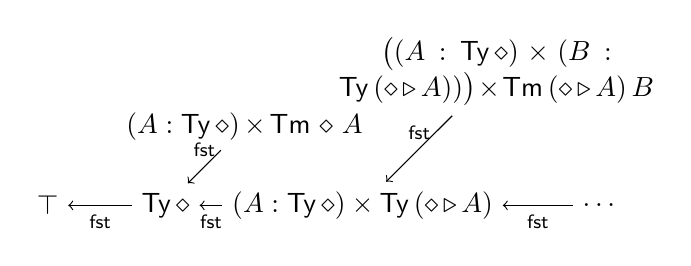
\begin{tikzpicture}
  \node (b0) at (0,0) {$\top$};
  \node (b1) at (1.5,0) {$\Ty\,\diamond$};
  \node (b2) at (4,0) {$(A:\Ty\,\diamond)\times\Ty\,(\diamond\ext A)$};
  \node (b3) at (7,0) {$\dots$};
  \node (c1) at (2.5,1) [text width=3cm] {$(A:\Ty\,\diamond)\times\Tm\,\diamond\,A$};
  \node (c2) at (5.7,1.7) [text width=4cm,align=center] {$\big((A:\Ty\,\diamond)\times(B:\Ty\,(\diamond\ext A))\big)\times\Tm\,(\diamond\ext A)\,B$};
  \draw[->,font=\scriptsize] (b1) edge node[below] {$\mathsf{fst}$} (b0);
  \draw[->,font=\scriptsize] (b2) edge node[below] {$\mathsf{fst}$} (b1);
  \draw[->,font=\scriptsize] (b3) edge node[below] {$\mathsf{fst}$} (b2);
  \draw[->,font=\scriptsize] (c1) edge node[above] {$\mathsf{fst}$} (b1);
  \draw[->,font=\scriptsize] (c2) edge node[above] {$\mathsf{fst}$} (b2);
\end{tikzpicture} \\
The substitution operation $\mathbb{S}$ for an element of
$x:\tilde{B}_{n+1}$ is a homomorphism of the slice B-frames
$\mathbb{B}/\partial(x) \ra \mathbb{B}/\mathsf{ft}(\partial(x))$. In
our notation, $x = (\Gamma, A, a)$ where $a : \Tm\,\Gamma\,A$, and the
homomorphism $\mathbb{S}$ corresponds to the following maps for the
bottom row of the diagram:
\begin{alignat*}{10}
  & \blank[\langle a\rangle] && : \Ty\,(\Gamma\ext A)\ra\Ty\,\Gamma \\
  & \blank[\langle a\rangle^+] && : \Ty\,(\Gamma\ext A\ext B)\ra\Ty\,(\Gamma\ext B[\langle a\rangle]) \\
  & \blank[\langle a\rangle^{++}] && : \Ty\,(\Gamma\ext A\ext B\ext C)\ra\Ty\,(\Gamma\ext B[\langle a\rangle]\ext C[\langle a\rangle^+]) \\
  & \dots,
\end{alignat*}
and similarly $\mathbb{S}$ also includes all the (lifted) substitution
operations for terms corresponding to the top row of the
diagram. Analogously, the weakening operation corresponds to
$\blank[\p^{+\dots+}]$ operations, and the generic element is $\q$ in
our notation. The six groups of equations correspond to our
$[\langle\rangle][]$, $[\p][^+]$, $\q[^+]$, $[\p][\langle\rangle]$,
$\q[\langle\rangle]$, $[\p^+][\langle\q\rangle]$ equations, in this
order. However we don't have the lifted versions of our equations,
equations $[\langle\rangle][]$, $[\p^+][\langle\q\rangle]$ are only
stated for types, and $\q[^+]$, $\q[\langle\rangle]$ are only stated
for terms. The missing equations are admissible, see Section
\ref{sec:admissible}. In the presence of universes and $\Pi$ types, we
reduce the needed equations even more, see Section
\ref{sec:minimisation}.

Kaposi and Luksa \cite{luksa} defined a telescopic single substitution
calculus for simple type theory, it can be seen as a simply typed
version of B-systems. They show that the category of contextual models
of their calculus is equivalent to the category of contextual simply
typed CwFs with function space. Their equivalence result holds even
without the presence of function space. In the presence of function
space, the same equivalence holds for the simply typed version of our
substitution calculus, see the formalisation accompanying this paper.

The first generalised algebraic presentation of type theory was Thomas
Ehrhard's calculus \cite{ehrhard,coquandEhrhard} which featured a
parallel substitution calculus with $\p$, $\blank^+$ and
$\langle\blank\rangle$ operations, just like in our calculus. Our
single substitution calculus is essentially Ehrhard's calculus with
the categorical composition and identity operations
removed. Categories with families (CwFs
\cite{DBLP:conf/types/Dybjer95,Castellan2021}) feature $\p$, $\q$,
$\blank,\blank$ operations which make it more apparent that
substitutions are lists of terms. CwFs are equivalent to Ehrhard's
calculus, and so are contextual categories/C-systems
\cite{DBLP:journals/apal/Cartmell86,DBLP:journals/lmcs/AhrensLV18},
the natural models of Awodey \cite{DBLP:journals/mscs/Awodey18} and
B-systems \cite{AHRENS_EMMENEGGER_NORTH_RIJKE_2023}.

Most computer formalisations of type theory are extrinsic
\cite{DBLP:journals/pacmpl/0001OV18,DBLP:conf/cpp/AdjedjLMPP24,DBLP:journals/jar/SozeauABCFKMTW20}:
they define the syntax as abstract syntax trees, and equip it with
typing and conversion relations. A higher level representation is
working in setoid hell \cite{chapman09eatitself}: terms are
intrinsically well-typed, but conversion is still an explicit
relation. For formalising the GAT-level syntax, one needs a stronger
metatheory than ordinary Agda or Coq: the metatheory has to support
quotient inductive-inductive types (QIITs
\cite{DBLP:journals/pacmpl/KaposiKA19}), in other words, initial
models of GATs. Altenkirch and Kaposi
\cite{DBLP:conf/popl/AltenkirchK16} formalised the syntax of type
theory using postulated QIITs in Agda, together with parametricity and
normalisation \cite{lmcs:4005} proofs. Brunerie and de Boer
\cite{initiality-agda} constructed the initial contextual category in
Agda using postulated quotients. QIITs are supported by the cubical
set model \cite{DBLP:conf/lics/CoquandHM18} and the setoid model
\cite{kaposi-qiit-setoid}, thus Cubical Agda
\cite{DBLP:journals/jfp/VezzosiMA21} and setoid/observational type
theory \cite{setoid,DBLP:phd/hal/Pujet22} support QIITs. For example,
in Cubical Agda, set-truncated and groupoid-truncated syntaxes of type
theory have been formalised \cite{cohtt}. Without QIITs, tricks such
as shallow embedding the syntax can be used to formalise metatheoretic
results about type theory such as gluing
\cite{kaposi_et_al:LIPIcs:2019:10532}, and its special cases
canonicity and parametricity \cite{kaposi-shallow}.

At the level of abstraction of SOGATs
\cite{uemura,DBLP:conf/fscd/KaposiX24}, the difference between single
and parallel substitution calculi are not visible. However, the
metatheory of type theory can be still investigated in this abstract
setting, via the methods of Synthethic Tait Computability
\cite{DBLP:phd/us/Sterling22} or internal sconing
\cite{DBLP:conf/fscd/BocquetKS23}.

% TODO: say that this is the paper version of the \cite{singleTypes}
% paper

\subsection{Metatheory and formalisation}

Our metatheory is observational type theory
\cite{DBLP:phd/hal/Pujet22} with quotient inductive-inductive types
(QIITs). On paper we usually omit writing coercions, so our notation
is close to extensional type theory. Sections \ref{sec:tt} and
\ref{sec:admissible} of this paper are formalised in the proof
assistant Agda, we use a strict Prop-valued
\cite{DBLP:journals/pacmpl/GilbertCST19} equality type with postulated
coercion rule (transport rule) and postulated QIITs with computation
rules added using rewrite rules
\cite{DBLP:journals/pacmpl/CockxTW21}. Our notation on paper is close
to Agda's, we write $\Pi$ types as $(x:A)\ra B$, $\Sigma$ types as
$(x:A)\times B$, and use implicit arguments and overloading
extensively.

\section{Single substitution syntax}
\label{sec:tt}

In this section, we introduce the syntax of type theory with function
space and universes in a minimalistic way, only introducing operations
that are unavoidable. We eschew boilerplate by only defining
well-formed, well-scoped, well-typed terms that are quotiented by
conversion. This means that the equalities that hold between terms are
the ways we can convert terms to each other when running them as
programs. We give a tutorial-style introduction to the syntax, we do
not assume prior knowledge of the metatheory of type theory. The
definition of type theory that we obtain is the same as the single
substitution GAT semantics \cite{DBLP:conf/fscd/KaposiX24} of the
SOGAT (\ref{eq:tt}).

First of all, we need a sort of terms which have to be indexed by
types because we only want well-typed terms. Both types and terms can
include variables, and to keep track of the currently available
variables, we also index them by contexts: a context is a list of
types, the length is the number of available variables, and we add new
variables at the end (that is, they are snoc-lists and not
cons-lists). Types are also indexed by their universe level, this is a
technical requirement for avoiding Russell's paradox. The index $i$ is
an implicit argument of $\Tm$.
\begin{alignat*}{10}
& \Con && : \Set \\
& \Ty && : \Con\ra\N\ra\Set \\
& \Tm && : (\Gamma:\Con)\ra\Ty\,\Gamma\,i\ra\Set
\end{alignat*}
Just as lists have two constructors, there are two ways to form
contexts: the empty context $\diamond$ and context extension $\ext$
which is like the snoc operation for lists. Context extension takes a
type which can have variables in the context preceeding the type.
\begin{alignat*}{10}
& \diamond && : \Con \\
& \blank\ext\blank && : (\Gamma:\Con)\ra\Ty\,\Gamma\,i\ra\Con
\end{alignat*}
We will refer to variables by their distance from the end of the
context. We would like to describe the operation providing the last
variable in a context, the zero De Bruijn index, we denote it by $\q :
\Tm\,(\Gamma\ext A)\,A'$. It is a term in an extended context, and it
should have type $A$, but the issue is that $A : \Ty\,\Gamma$, and $A'
: \Ty\,(\Gamma\ext A)$. We need a way to weaken the type $A$ to obtain
such an $A'$. For this, we will introduce an operation $\blank[\p] :
\Ty\,\Gamma\,i\ra\Ty\,(\Gamma\ext A)\,i$ and define $A' := A[\p]$. Instead
of introducing just $\blank[\p]$, we generalise a bit and add a new
sort $\Sub$ which for now only has the single element $\p$ and the
operation $\blank[\blank]$ is called \emph{instantiation}. We
instantiate the type with the weakening in
$\Sub\,\Delta\,\Gamma$. Elements of $\Sub$ will be in general called
substitutions, hence the name, but for now, we only have single end-of
context weakenings in $\Sub$. $\Delta$ is called the domain, $\Gamma$
the codomain of a $\Sub\,\Delta\,\Gamma$.
\begin{alignat*}{10}
& \Sub && : \Con\ra\Con\ra\Set \\
& \p && : \Sub\,(\Gamma\ext A)\,\Gamma \\
& \blank[\blank] && : \Ty\,\Gamma\,i\ra\Sub\,\Delta\,\Gamma\ra\Ty\,\Delta\,i \\
& \q && : \Tm\,(\Gamma\ext A)\,(A[\p])
\end{alignat*}
The operations $\p$ and $\q$ take three implicit parameters, $\Gamma$,
$i$ and $A$, while $\blank[\blank]$ takes $\Gamma$, $i$ and $\Delta$
implicitly. Still, we only have the last variable $\q$ in the context,
we don't have e.g.\ the last but one variable in $\Tm\,(\Gamma\ext
A\ext B)\,(A[\p][\p])$ where we had to weaken $A$ twice to make it fit
with its context. To obtain more variables, we also allow weakening of
terms, more precisely, we introduce an instantiation operation for
terms with an overloaded notation.
\begin{alignat*}{10}
& \blank[\blank] && : \Tm\,\Gamma\,A\ra(\gamma:\Sub\,\Delta\,\Gamma)\ra\Tm\,\Delta\,(A[\gamma])
\end{alignat*}
Note that this is a dependent function as the type of the resulting
term has to be weakened the same way as the term itself. Now we can
define all variables counting from the end of the context (De Bruijn
indices \cite{debruijn}): $0 := \q$, $1 := \q[\p]$, $2 := \q[\p][\p]$,
$3 := \q[\p][\p][\p]$, and so on.

Next we add dependent function space $\Pi$: the domain of a dependent
function is a type in some context $\Gamma$, and the codomain can also
refer to a variable in the domain, so we extend the context of the
codomain type with the type of the domain. For simplicity, both types
are at the same level (this can be remedied using $\Lift$, see later).
\begin{alignat*}{10}
& \Pi && : (A:\Ty\,\Gamma\,i)\ra\Ty\,(\Gamma\ext A)\,i\ra\Ty\,\Gamma\,i
\end{alignat*}
The nondependent function space $\blank\Ra\blank :
\Ty\,\Gamma\,i\ra\Ty\,\Gamma\,i\ra\Ty\,\Gamma\,i$ is a special case of $\Pi$
and we define it as the abbreviation $A\Ra B := \Pi\,A\,(B[\p])$.

Because we introduced weakening, we now have to explain what happens
to a $\Pi$ type once we weaken it. Assume $A : \Ty\,\Gamma\,i$,
$B:\Ty\,(\Gamma\ext A)\,i$ and we have $\p:\Sub\,(\Gamma\ext
C)\,\Gamma$. Then we say $(\Pi\,A\,B)[\p] = \Pi\,(A[\p])\,(B[\p'])$,
but $B$ cannot be weakened by $\p$ because there we need $\p' :
\Sub\,(\Gamma\ext C\ext A[\p])\,(\Gamma\ext A)$. So $p'$ has to be a
new kind of weakening which adds a new variable in the last but one
position. But then we need an equation also for $(\Pi\,A\,B)[\p']$,
introducing a new weakening which adds a new variable in the last but
two position, and so on. We solve all of these issues by allowing the
\emph{lifting} of a weakening: $\gamma^+$ will be the same as the
weakening $\gamma : \Sub\,\Delta\,\Gamma$, except that it will add an
extra variable both at the end of the domain and codomain
context.
\begin{alignat*}{10}
& \blank^+ && : (\gamma:\Sub\,\Delta\,\Gamma)\ra\Sub\,(\Delta\ext A[\gamma])\,(\Gamma\ext A)
\end{alignat*}
Note that $A$ is an implicit argument of $\blank^+$, and that it has
to be instantiated by the weakening $\gamma$ in the domain context in
order to fit in. Now we can explain how instantiation acts on $\Pi$ by
the following equation.
\begin{alignat*}{10}
& \Pi[] && : (\Pi\,A\,B)[\gamma] = \Pi\,(A[\gamma])\,(B[\gamma^+])
\end{alignat*}
The above equation has 6 implicit arguments, namely $\Gamma$, $i$,
$A$, $B$, $\Delta$ and $\gamma$.  This rule works for any weakening,
no matter how many $\blank^+$s have been applied to it. As of now, all
elements of $\Sub$ have the form
\begin{alignat*}{10}
  & \p^{+^n} : \Sub\, && (\Gamma\ext A\ext B_1[\p]\ext B_2[\p^+]\ext\dots\ext B_n[\p^{+^{n-1}}]) \\
  & && (\Gamma\ext B_1\ext B_2\ext\dots\ext B_n).
\end{alignat*}
where $+^n$ means the $n$-times iteration of $\blank^+$.

Now that we have weakenings of the form $\gamma^+$, we have to say how
they act on variables, that is, terms of the form
$\q[\p]\dots[\p]$. We express this using two rules: we say what
$\q[\gamma^+]$ computes to, and what $b[\p][\gamma^+]$ computes to
where $b$ is an arbitrary term. $\q[\gamma^+]$ should be the same as
$\q$ (with different implicit arguments as the $\q$ in
$\q[\gamma^+]$), as the weakening happens somewhere in the middle of
the context, so the index of the variable remains unchanged. However,
assuming $\q:\Tm\,(\Gamma\ext A)\,(A[\p])$, we have $\q[\gamma^+] :
\Tm\,(\Delta\ext A[\gamma])\,(A[\p][\gamma^+])$, but in the same
context, we have $\q : \Tm\,(\Delta\ext A[\gamma])\,(A[\gamma][\p])$,
hence the terms in the two sides of the equation $\q[\gamma^+] = \q$
have different types. But these two types should be the same:
weakening a type at the end of the context, and then applying another
lifted weakening should be the same as first weakening somewhere and
then weakening at the end. We first assume this equation for types,
then the equation $\q[\gamma^+] = \q$ becomes well-typed (in the
metatheory). The equation for $b[\p][\gamma^+]$ has the same shape as
the newly assumed rule for types. Thus we add the following three
equations.
\begin{alignat*}{10}
& [\p][^+] && : B[\p][\gamma^+] = B[\gamma][\p] \\
& [\p][^+] && : b[\p][\gamma^+] = b[\gamma][\p] \\
& \q[^+] && : \q[\gamma^+] = \q
\end{alignat*}
The second and third equations only make sense because of the first
equation. The phenomenon that later equations (or operations) depend
on previous equations is usual in the world of GATs. In fact, the
later equations cannot even be stated without having some previous
equations.

Now that we have $[\p][^+]$ for types, we can derive the instantiation
rule for nondependent function space as follows.
\begin{alignat*}{10}
  & (A\Ra B)[\gamma] && {=} \\
  & (\Pi\,A\,(B[\p]))[\gamma] && {=}(\Pi[]) \\
  & \Pi\,(A[\gamma])\,(B[\p][\gamma^+])\,\, && {=}([\p][^+]) \\
  & \Pi\,(A[\gamma])\,(B[\gamma][\p]) && {=} \\
  & (A[\gamma])\Ra(B[\gamma])
\end{alignat*}

So far our only terms are variables, but we would like to define
functions via lambda abstraction. Abstraction takes a term in a
context extended by the domain of the function. It comes with a rule
for instantiation analogous to $\Pi[]$.
\begin{alignat*}{10}
& \lam && : \Tm\,(\Gamma\ext A)\,B\ra\Tm\,\Gamma\,(\Pi\,A\,B) \\
& \lam[] && : (\lam\,b)[\gamma] = \lam\,(b[\gamma^+])
\end{alignat*}
Note that the equation $\lam[]$ only makes sense because of the
previous equation $\Pi[]$: the left hand side is in
$\Tm\,\Delta\,(\Pi\,A\,B[\gamma])$, in the right hand side,
$t[\gamma^+] : \Tm\,(\Delta\ext A[\gamma])\,(B[\gamma^+])$, hence the
right hand side is in
$\Tm\,\Delta\,(\Pi\,(A[\gamma])\,(B[\gamma^+]))$.

The functions $\lambda x.x$ and $\lambda x\,y.x$ can be defined in our
syntax as $\lam\,\q : \Tm\,\Gamma\,(A\Ra A)$ and
$\lam\,(\lam\,(\q[\p])) :
\Tm\,\Gamma\,\big(\Pi\,A\,(B\Ra(A[\p]))\big)$ which make sense for all
$\Gamma$, $A$, $B$.

The application operation for dependent function space is a bit
tricky, because the return type depends on the input: the argument of
the function will appear in the return type. We write application by
an infix $\blank\cdot\blank :
\Tm\,\Gamma\,(\Pi\,A\,B)\ra(a:\Tm\,\Gamma\,A)\ra\Tm\,\Gamma\,B'$,
where $B' : \Ty\,\Gamma$ should be $B:\Ty\,(\Gamma\ext A)$ where the
last variable is \emph{substituted} (instantiated) by $a$. For this,
we introduce a new element of $\Sub$ called single substitution which
goes the opposite way of $\p$. Now we can use instantiation
$\blank[\blank]$ to substitute the last variable in $B$.
\begin{alignat*}{10}
& \langle\blank\rangle && : \Tm\,\Gamma\,A\ra\Sub\,\Gamma\,(\Gamma\ext A) \\
& \blank\cdot\blank && : \Tm\,\Gamma\,(\Pi\,A\,B)\ra(a:\Tm\,\Gamma\,A)\ra\Tm\,\Gamma\,(B[\langle a\rangle])
\end{alignat*}
We could have introduced new, separate sorts and $\blank[\blank]$
operations for weakenings and substitutions, but we merge them for
simplicity. There is no need for separation: just as weakenings can be
lifted, single substitutions can also be lifted, and the
weakening-rules $\Pi[]$, $\lam[]$ also work for single
substitutions. We won't have more ways to introduce elements of
$\Sub$, and there are no equations on $\Sub$. An element of $\Sub$ is
either a single weakening $\p$ lifted a couple of times, or a single
substitution lifted a couple of times. We call elements of $\Sub$
substitutions for simplicity.

With the introduction of $\blank\cdot\blank$, we need a new
substitution rule, but again it only makes sense with an extra
equation on types saying that first substituting the last variable and
then an arbitrary substitution is the same as first the lifted version
of the arbitrary substitution that does not touch the last variable,
and then substituting the last variable.
\begin{alignat*}{10}
& [\langle\rangle][] && : B[\langle a\rangle][\gamma] = B[\gamma^+][\langle a[\gamma]\rangle] \\
& {\cdot}[] && : (t\cdot a)[\gamma] = (t[\gamma])\cdot(a[\gamma])
\end{alignat*}
Following the introduction of the operation $\langle\blank\rangle$, we
need to explain how it acts on variables. Given a variable in the
middle of the context (a term $b[\p]$), substituting its last variable
simply returns $b$. Substituting the last variable $\q$ reads out the
term from $\langle\blank\rangle$. As usual, the rules only typecheck
if we have an equation for types.
\begin{alignat*}{10}
& [\p][\langle\rangle] && : B[\p][\langle a\rangle] = B \\
& [\p][\langle\rangle] && : b[\p ][\langle a\rangle] = b \\
& \q[\langle\rangle] && : \q[\langle a\rangle] = a
\end{alignat*}
We don't have a separate sort of variables, so the rule
$[\p][\langle\rangle]$ holds not only for variables, but for arbitrary
terms. This is not an issue, as weakening a term at the end of its
context, and then substituting the newly introduced variable is the
same as not doing anything.

We add the computation and uniqueness rule for function space, where
the uniqueness rule again needs an extra equation on the codomain type
of the function to make sense. This is the typal version of the
equation mentioned in the introduction.
\begin{alignat*}{10}
& \Pi\beta && : \lam\,b\cdot a = b[\langle a\rangle] \\
& [\p^+][\langle\q\rangle] && : B[\p^+][\langle\q\rangle] = B \\
& \Pi\eta && : t = \lam\,(t[\p]\cdot\q)
\end{alignat*}

We add the rules for universes. A universe is a type containing codes
for types, this is witnessed by $\El$ (elements) and $\cd$ (code),
which make an isomorphism between terms of type $\U\,i$ and types of
level $i$. All three operations come with substitution rules ($\El[]$
and $\cd[]$ are interderivable, so it would be enough to assume one of
the two, but we add both to completely align with the algorithm
\cite{DBLP:conf/fscd/KaposiX24} generating the rules from the SOGAT
(\ref{eq:tt})).
\begin{alignat*}{10}
  & \U && : (i:\N)\ra\Ty\,\Gamma\,(1+i)\hspace{2em} && \U[] && : (\U\,i)[\gamma] = \U\,i \\
  & \El && : \Tm\,\Gamma\,(\U\,i) \ra \Ty\,\Gamma\,i && \El[] && : (\El\,\hat{A})[\gamma] = \El\,(\hat{A}[\gamma]) \\
  & \cd && : \Ty\,\Gamma\,i\ra\Tm\,\Gamma\,(\U\,i) && \cd[] && : (\cd\,A)[\gamma] = \cd\,(A[\gamma]) \\
  & \U\beta && : \El\,(\cd\,A) = A \\
  & \U\eta && : \cd\,(\El\,\hat{A}) = \hat{A}
\end{alignat*}
Finally, we add the rules for moving types one level up. Because we
defined function space only between types at the same level, without
lifting, we cannot even define the polymorphic identity function.
\begin{alignat*}{10}
  & \Lift && : \Ty\,\Gamma\,i\ra\Ty\,\Gamma\,(1+i)\hspace{3.5em} && (\Lift\,A)[\gamma] = \Lift\,(A[\gamma]) \\
  & \mk && : \Tm\,\Gamma\,A \ra \Tm\,\Gamma\,(\Lift\,A) && (\mk\,a)[\gamma] = \mk\,(a[\gamma]) \\
  & \un && : \Tm\,\Gamma\,(\Lift\,A) \ra \Tm\,\Gamma\,A && (\un\,a)[\gamma] = \un\,(a[\gamma]) \\
  & \Lift\beta && : \un\,(\mk\,a) = a \\
  & \Lift\eta && : \mk\,(\un\,a) = a
\end{alignat*}
\begin{definition}[Single substitution calculus with $\Pi$, $\U$, $\Lift$]\label{def:tt}
This concludes the first-order single substitution semantics of the
SOGAT (\ref{eq:tt}). For reference, we list the same rules again in
Appendix \ref{app:tt}.
\end{definition}
The theory can be extended with new type and term formers in the same
fashion: each rule has to be indexed over arbitrary contexts and come
equipped with a substitution rule. There is no need to add more
structural (substitution calculus) rules. For example, we show how to
extend Definition \ref{def:tt} with the SOGAT-rules (\ref{eq:sigma}).
\begin{definition}[Single substitution calculus with $\Pi$, $\U$, $\Lift$, $\top$, and $\Sigma$ types]\label{def:sigma}
  We extend Definition \ref{def:tt} with the following rules.
  \begin{alignat*}{10}
    & \top && : \Ty\,\Gamma\,0 && \top[] && : \top[\gamma] = \top \\
    & \tt && : \Tm\,\Gamma\,\top && \tt[] && : \tt[\gamma] = \tt \\
    & \top\eta && : t = \tt \\
    & \Sigma && : (A:\Ty\,\Gamma\,i)\ra\Ty\,(\Gamma\ext A)\,i\ra\Ty\,\Gamma\,i \\
    & \Sigma[] && : (\Sigma\,A\,B)[\gamma] = \Sigma\,(A[\gamma])\,(B[\gamma^+]) \\
    & \fst,\snd && : \Tm\,\Gamma\,(\Sigma\,A\,B)\cong \\
    & && \rlap{$\hphantom{{}:{}} (a:\Tm\,\Gamma\,A)\times\Tm\,\Gamma\,(B[\langle a\rangle]) : (\blank,\blank)$} \\
    & {,}[] && : (a,b)[\gamma] = (a[\gamma],b[\gamma])
  \end{alignat*}
  To save space, we compressed the introduction, elimination, $\beta$
  and $\eta$ rules for $\Sigma$ into one isomorphism, and did not list
  substitution laws for $\fst$ and $\snd$ as they are derivable.
\end{definition}

\subsection{Examples}

The polymorphic identity function for types at the level 0 is defined
as
\[
\lam\,(\lam\,\q) : \Tm\,\diamond\,\Big(\Pi\,(\U\,0)\,\big(\Lift\,(\El\,\q)\Ra\Lift\,(\El\,\q)\big)\Big).
\]
Note that readability of this term essentially relies on implicit
arguments. For example, $\q$ takes $(\diamond\ext\U\,0)$ as its first,
$1$ as its second and $\Lift\,(\El\,\q)$ as its third implicit
argument, and these arguments themselves are terms written using
implicit arguments. Inrinsically typed terms are the same as
derivation trees, we illustrate this by deriving this term as follows.
\[
\infer[\text{(*)}]{\lam\,(\lam\,\q) : \Tm\,\diamond\,\big(\Pi\,(\U\,0)\,(\Lift\,(\El\,\q)\Ra\Lift\,(\El\,\q))\big)}{\infer{\lam\,\q : \Tm\,(\diamond\ext\U\,0)\,(\Lift\,(\El\,\q)\Ra\Lift\,(\El\,\q))}{\infer{\q : \Tm\,(\diamond\ext\U\,0\ext\Lift\,(\El\,\q))\,(\Lift\,(\El\,\q)[\p])}{}}}
\]
Note that in step (*), $\lam$ made it sure that $\U\,0$ and
$\Lift\,(\El\,\q)\Ra\Lift\,(\El\,\q)$ are types at the same level,
this is why we had to lift $\El\,\q$. Another subtle thing is
happening when deriving the third implicit argument of $\q$. We have
to coerce $\q$ along the equality $\U[]$.
\[
\infer{\Lift\,(\El\,\q) : \Ty\,(\diamond\ext\U\,0)\,1}{\infer{\El\,\q : \Ty\,(\diamond\ext\U\,0)\,0}{\infer{\q : \Tm\,(\diamond\ext\U\,0)\,(\U\,0)}{\infer{\q : \Tm\,(\diamond\ext\U\,0)\,((\U\,0)[\p])}{} && \infer{\U[] : (\U\,0)[\p] = \U\,0}{}}}}
\]
When working informally (or in extensional type theory), we don't
write the coercion, but Agda requires it.

Given a type $A:\Ty\,\diamond\,0$, and $a : \Tm\,\diamond\,A$, we have
\begin{alignat*}{10}
  & \lam\,(\lam\,\q)\cdot\cd\,A\cdot a && {=}(\Pi\beta) \\
  & (\lam\,\q[\langle\cd\,A\rangle])\cdot a && {=}(\lam[]) \\
  & (\lam\,(\q[\langle\cd\,A\rangle^+]))\cdot a && {=}([\q][^+]) \\
  & (\lam\,\q)\cdot a && {=}(\Pi\beta) \\
  & \q[\langle a\rangle] && {=}(\q[\langle\rangle]) \\
  & a
\end{alignat*}
If we want to specify open inputs $A':\Ty\,(\diamond\ext C)\,0$, and
$a' : \Tm\,(\diamond\ext C)\,A'$, we have to weaken our function to
accept them:
\begin{alignat*}{10}
  & \lam\,(\lam\,\q)[\p] : \Tm\,&& (\diamond\ext C)\,\\
  & && \Big(\Pi\,(\U\,0)\,\big(\Lift\,(\El\,\q)\Ra\Lift\,(\El\,\q)\big)[\p]\Big)
\end{alignat*}
But we have
\[
\lam\,(\lam\,\q)[\p] \overset{\lam[]\,2\text{x}}{=} \lam\,(\lam\,(\q[\p^{++}])) \overset{\q[^+]}{=} \lam\,(\lam\,\q)
\]
(with different implicit arguments), so we are able apply $\cd\,A'$
and $a'$ just as before. What we cannot do is to directly weaken a
term in context $\diamond$ to an arbitrary metavariable context
$\Gamma$, we can only do this step by step by applying weakening
$\blank[\p]$ for each type in the context.

As a sanity check for our notion of SSC-model, we defined the standard
(metacircular \cite{DBLP:conf/popl/AltenkirchK16}) model of the
SSC-based calculus calculus in Agda. We used the techniques of Kovács
\cite{DBLP:conf/csl/Kovacs22} to define inductive-recursive universes
to model the infinite hierarchy of types, and all the SSC-equations
hold by reflexivity in this model. We defined the analogous CwF-based
standard model.

\section{Admissible equations}
\label{sec:admissible}

TODO: say that we assume the QIIT version of this.

$\alpha$-normal forms could also be called substitution normal forms.

In this section we show that a category with families (CwF) equipped
with a hierarchy of Coquand-universes and $\Pi$ types can be derived
from the single substitution syntax defined in \autoref{sec:tt}.

TODO: show that the SSC operations are derivable from CwF.

We conjecture that the same works for any SOGAT.

\section{stuff}

The following four equations correspond to equations in B-systems which cannot
be derived from the equations of SSC, these are versions of equations in section
\ref{sec:tt} lifted under arbitrary amount of $\blank^+$s.
\begin{equation}\label{eq:lifted}
\begin{aligned}
  B[\p^{+^n}][(\gamma^+)^{+^n}] & = B[\gamma^{+^n}][\p^{+^n}] \\
  B[\p^{+^n}][\langle a \rangle^{+^n}] & = B \\
  B[\langle a \rangle^{+^n}][\gamma^{+^n}] & = B[(\gamma^+)^{+^n}][\langle a[\gamma] \rangle^{+^n}] \\
  B[(\p^+)^{+^n}][\langle\q\rangle^{+^n}] & = B
\end{aligned}
\end{equation}
The correspoinding equations on terms are also needed. Note that we do not have
the non-lifted term versions of the last two equations in SSC.

To formally state the equations in (\ref{eq:lifted}), we define telescopes as an
inductive type together with a recursive operation to append telescopes to
contexts.
\begin{alignat*}{10}
  & \Tel && : \Con\ra\Set \\
  & \blank+\blank && : (\Gamma:\Con)\ra\Tel\,\Gamma\ra\Con \\
  & \diamond && : \Tel\,\Gamma \\
  & \blank\ext\blank && : (\Omega:\Tel\,\Gamma)\ra\Ty\,(\Gamma+\Omega)\ra\Tel\,\Omega
\end{alignat*}
The appending operation is defined recursively on telescopes.
\begin{alignat*}{10}
  & \Gamma+\diamond && := \Gamma \\
  & \Gamma+(\Omega\ext A) && := (\Gamma+\Omega)\ext A
\end{alignat*}
We then define a lifting operation over any telescope mutually with an
instantiation operation on telescopes by recursion on telescopes.
\begin{alignat*}{10}
  & \blank[\blank] && : \Tel\,\Gamma\ra\Sub\,\Delta\,\Gamma\ra\Tel\,\Delta \\
  & \blank^{+^\Omega} && : (\gamma:\Sub\,\Delta\,\Gamma)\ra\Sub\,(\Delta+\Omega[\gamma])\,(\Gamma+\Omega)
\end{alignat*}

If we try to prove the equations in (\ref{eq:lifted}) by induction on the types
and terms, we run into difficulties in the instantiation case, as we would have
to commute the instantiations without the equations to do so. Therefore, we
first $\alpha$-normalize the syntax to compute away all the instantiations, then
prove the equations by induction on the $\alpha$-normal forms.

A type or term is $\alpha$-normal if it does not contain instantiation
operations, except at the leaves of the syntax tree as variables. However,
$\alpha$-normal terms can still contain $\beta$/$\eta$ redexes, so that we do
not need to do full normalization. We define variables and $\alpha$-normal forms
as inductive predicates in $\Prop$.
\begin{itemize}
  \item $\q:\Tm\,(\Gamma\ext A)\ (A[\p])$ is a variable.
  \item $x[\p]:\Tm\,(\Gamma\ext A)\ (B[\p])$ is a variable if $x:\Tm\,\Gamma\,B$
  is a variable.
  \item $x:\Tm\,\Gamma\,A$ is $\alpha$-normal if $x$ is a variable.
  \item $\Pi\,A\,B:\Ty\,\Gamma\,i$ is $\alpha$-normal if $A$ and $B$ are
  $\alpha$-normal types.
  \item $\app\,f\,a:\Tm\,\Gamma\,(B[\langle a \rangle])$ is $\alpha$-normal if
  $A$ and $B$ are $\alpha$-normal types, $f:\Tm\,\Gamma\,(\Pi\,A\,B)$ and
  $a:\Tm\,\Gamma\,A$ are $\alpha$-normal terms.
\end{itemize}
The predicate is defined similarly for the other type and term formers. Notably,
we do not state that instantiated types/terms are $\alpha$-normal. It is
important to truncate the $\alpha$-normal predicates to be propositions to
ensure that it preserves the $\beta$/$\eta$ conversion rules.

We prove that the $\alpha$-normal predicate holds for $\alpha$-normal types and
terms instantiated with $\alpha$-normal substitutions. However, this needs to be
proved separately for weakenings and $\alpha$-normal single substitutions for
the induction to be well-founded. We define predicates for weakening and
$\alpha$-normal single substitutions as follows.
\begin{itemize}
  \item $\p$ is a weakening.
  \item $\gamma^+$ is a weakening if $\gamma$ is a weakening.
  \item $\langle a \rangle$ is an $\alpha$-normal single substitution if $a$ is an
  $\alpha$-normal term.
  \item $\gamma^+$ is an $\alpha$-normal single substitution if $\gamma$ is an
  $\alpha$-normal single substitution.
\end{itemize}

\begin{lemma}
  \label{thm:alpha}
  The $\alpha$-normal predicate holds for any type and term.
\end{lemma}
\begin{proof}
  By induction on the syntax, $\alpha$-normalizing the substitutions at the same
  time.
\end{proof}

Instead of doing induction on $\alpha$-normal forms for each of the equations in
(\ref{eq:lifted}), we define a general lemma which can lift any equation between
instantiations over a telescope. For this we define $\Sub^*$ to be $\Sub$ with
freely added identity and composition operations, we do not require it to
satisfy the laws of a category as we will not compare $\Sub^*$s directly for
equality, only between types and terms instantiated with $\Sub^*$s. All
instantiation operations, lifting operations, and substitution rules can be
redefined for $\Sub^*$.
\begin{lemma}
  \label{thm:lifting}
  Given and $\sigma, \delta : \Sub^*\,\Delta\,\Gamma$, if $A[\sigma] =
  A[\delta]$ and $x[\sigma] = x[\delta]$ for any $A:\Ty\,\Gamma$ and variable
  $x:\Tm\,\Gamma\,A$, then
  \begin{itemize}
    \item $\Omega[\sigma] = \Omega[\delta]$ for $\Omega:\Tel\,\Gamma$
    \item $A[\sigma^{+^\Omega}] = A[\delta^{+^\Omega}]$ for $A:\Ty\,(\Gamma+\Omega)$
    \item $a[\sigma^{+^\Omega}] = a[\delta^{+^\Omega}]$ for $a:\Tm\,(\Gamma+\Omega)\,A$
  \end{itemize}
  Note that the later equations depend the the earlier ones.
\end{lemma}
\begin{proof}
  Assuming the first equation, we prove that $x[\sigma^{+^\Omega}] =
  x[\delta^{+^\Omega}]$ for any variable $x$ by induction on the telescope and
  the variable. Then the two latter equations can be proven by mutual induction
  on $\alpha$-normalized types and terms, still assuming the first equation.
  Finally we prove the first equation by induction on the telescope, using the
  previously proven equation for types, discharging its assumption.
\end{proof}

We can simulate parallel substitutions using $\Sub^*$ as iterated single
substitutions, however it does not satisfy the equations of parallel
substitutions. Thus we define parallel substitutions as a list of terms with a
map into $\Sub^*$, and reuse instantiation operation of $\Sub^*$ to convert it
into a sequence of instantiations of single substitutions.
\begin{alignat*}{10}
  & \Tms && : \Con\ra\Con\ra\Con \\
  & \llcorner\blank\lrcorner && : \Tms\,\Delta\,\Gamma \to \Sub^*\,\Delta\,\Gamma \\
  & \epsilon && : \Tms\,\Gamma\,\diamond \\
  & \blank,\blank && : (\gamma:\Tms\,\Delta\,\Gamma)\ra\Tm\,\Delta\,(A[\llcorner\gamma\lrcorner])\ra\Tms\,\Delta\,(\Gamma\ext A) \\
  & \llcorner\epsilon\lrcorner && := \id\circ\p\circ\dots\circ\p \\
  & \llcorner\gamma,a\lrcorner && := \llcorner\gamma\lrcorner^+\circ\langle a \rangle
\end{alignat*}
The computation of instantiating with $\Tms$ is illustrated below.
\begin{gather*}
  B[\llcorner\epsilon,a_1,a_2,\dots,a_{n-1},a_n\lrcorner] = \\
  B[\p^{+^n}]\dots[\p^{+^n}][\langle a_1 \rangle^{+^{n-1}}][\langle a_2 \rangle^{+^{n-2}}]\dots[\langle a_{n-1} \rangle^+][\langle a_n \rangle]
\end{gather*}
All CwF operations and equations can be defined with $\Tms$ by induction.

\begin{theorem}
  Contexts, types, and terms in the SSC syntax are isomorphic to the
  corresponding sorts in the CwF syntax.
\end{theorem}
\begin{proof}\leavevmode
  \begin{description}
    \item[$\Rightarrow$] By recursion on the syntax, SSC operations can be
    trivially interpreted by CwF operations.
    \item[$\Leftarrow$] By recursion on the syntax, using $\Tms$ to interpret
    parallel substitutions.
  \end{description}
  The roundtrips are proven by induction on the syntax.
\end{proof}

\section{Minimisation}
\label{sec:minimisation}

In this section we show that if have we universes and $\Pi$ types
(which is the case in the theory (\ref{eq:tt})), we can decrease the
number of equations.

In our single substitution calculus, we have equation $[\p][^+]$
stated both for types and terms (we know that the left one is about
types because of our convention that type metavariables are uppercase
Latin letters and term metavariables are lowercase):
\[
B[\p][\gamma^+] = B[\gamma][\p] \hspace{4em} b[\p][\gamma^+] =_{[\p][^+]} b[\gamma][\p]
\]
We even need the first equation to typecheck the second one. We made
the dependency explicit by adding a subscript of the equality in the
equation for terms (in Agda, this dependency has to be made
explicit). An alternative presentation of the second equation without
requiring the first one is the following:
\[
[\p][^+]' : (e : B[\p][\gamma^+] = B[\gamma][\p])\ra b[\p][\gamma^+] =_{e} b[\gamma][\p]
\]
That is, for any type $B$ for which $B[\p][\gamma^+] = B[\gamma][\p]$,
we have that for any $b$ we have the equation (suitably over the input
equation). Thus we add a conditional equation.

It turns out that if we have Coquand-universes, the conditional
$[\p][^+]'$ rule is enough: the input equation holds for $B := \U\,i$
via $\U[]$, thus we get that for any $\hat{A} : \Tm\,\Gamma\,(\U\,i)$,
$\hat{A}[\p][\gamma^+] = \hat{A}[\gamma][\p]$. But every type has a
code in the universe, so for a $B : \Ty\,\Gamma\,i$,
\begin{alignat*}{10}
  & B[\p][\gamma^+] && {=}(\U\beta) \\
  & \El\,(\cd\,B)[\p][\gamma^+] && {=}(\El[]) \\
  & \El\,((\cd\,B)[\p][\gamma^+])\,\, && {=}([\p][^+]'\,\U[]) \\
  & \El\,((\cd\,B)[\gamma][\p]) && {=}(\El[]) \\
  & \El\,(\cd\,B)[\gamma][\p] && {=}(\U\beta) \\
  & B[\gamma][\p].
\end{alignat*}
Equation $[\q][^+] : \q[\gamma^+] = \q$ also only makes sense if we
have $[\p][^+]$ for types, so either we have to make $[\q][^+]$
conditional, or we coerce it along the derived equation.

We play the exact same game with $[\p][\langle\rangle]$: we replace it
with the conditional equation
\[
[\p][\langle\rangle]' : (e:B[\p][\langle a\rangle] = B)\ra b[\p][\langle a\rangle] =_e b,
\]
notice that we have the input for $B = \U\,i$, and derive the input
equation for all types. We make $\q[\langle\rangle]$ conditional as
well.

Now we turn our attention to the equation
\[
  [\langle\rangle][] : B[\langle a\rangle][\gamma] = B[\gamma^+][\langle a[\gamma]\rangle].
\]
We were forced to introduce it so that we can state the substitution
rule for function application $\cdot[]$. What if we made $\cdot[]$
itself conditional?
\begin{alignat*}{10}
  & \cdot[]' :{} && (e : B[\langle a\rangle][\gamma] = B[\gamma^+][\langle a[\gamma]\rangle])\ra \\
  & && (t\cdot a)[\gamma] =_e (t[\gamma])\cdot(a[\gamma])
\end{alignat*}
Again, for $B = \U$ we have the assumption $e$. But then $t$ is in
$\Tm\,\Gamma\,(\Pi\,A\,\U)$, which is isomorphic to $\Ty\,(\Gamma\ext
A)$. So we argue as follows for any $B : \Ty\,(\Gamma\ext A)$.
\begin{alignat*}{10}
  & B[\langle a\rangle][\gamma] && {=}(\U\beta) \\
  & \El\,(\cd\,(B[\langle a\rangle][\gamma])) && {=}(\cd[]) \\
  & \El\,((\cd\,B)[\langle a\rangle][\gamma]) && {=}(\Pi\beta) \\
  & \El\,((\lam\,(\cd\,B)\cdot a)[\gamma]) && {=}(\cdot[]'\,\U[]) \\
  & \El\,((\lam\,(\cd\,B)[\gamma])\cdot (a[\gamma]))\,\, && {=}(\lam[]) \\
  & \El\,(\lam\,(\cd\,B[\gamma^+])\cdot (a[\gamma])) && {=}(\Pi\beta) \\
  & \El\,(\cd\,B[\gamma^+][\langle a[\gamma]\rangle]) && {=}(\cd[]) \\
  & \El\,(\cd\,B)[\gamma^+][\langle a[\gamma]\rangle] && {=}(\U\beta) \\
  & B[\gamma^+][\langle a[\gamma]\rangle]
\end{alignat*}
Hence, the conditional $\cdot[]'$ equation implies the condition for
all types.

Finally, we will remove equation $[\p^+][\langle\q\rangle]$ by making
$\Pi\eta$ conditional. This needs another change: we substitute
$\Pi\beta$ for a more general variant which is also conditional on the
same equation.
\begin{alignat*}{10}
  & \Pi\eta' && : (e:B[\p^+][\langle\q\rangle] = B)\ra t =_e \lam\,(t[\p]\cdot\q) \\
  & \Pi\beta' && : (e:B[\p^+][\langle\q\rangle] = B)\ra (\lam\,b)[\p]\cdot\q =_e b
\end{alignat*}
But first we need to check that the usage of $\Pi\beta$ above when
proving $B[\langle a\rangle][\gamma] = B[\gamma^+][\langle
  a[\gamma]\rangle]$ is derivable from $\Pi\beta'$. Assuming a
$\hat{B} : \Tm\,(\Gamma\ext A)\,\U$,
\begin{alignat*}{10}
  & \Pi\beta^\U :{} &&  \lam\,\hat{B}\cdot a && {=}(\q[\langle\rangle]) \\
  & && \lam\,\hat{B}\cdot(\q[\langle a\rangle])\,\, && {=}([\p][\langle\rangle]) \\
  & && ((\lam\,\hat{B})[\p][\langle a\rangle])\cdot(\q[\langle a\rangle])\,\, && {=}(\cdot[]'\,\U[]) \\
  & && ((\lam\,\hat{B})[\p]\cdot\q)[\langle a\rangle] && {=}(\Pi\beta'\,\U[]) \\
  & && \hat{B}[\langle a\rangle].
\end{alignat*}
Now we derive the assumption of $\Pi\beta/\eta'$ for any type $B : \Ty\,(\Gamma\ext A)$.
\begin{alignat*}{10}
  & B[\p^+][\langle\q\rangle] && {=}(\U\beta) \\
  & \El\,(\cd\,B)[\p^+][\langle\q\rangle] && {=}(\El[]) \\
  & \El\,(\cd\,B[\p^+][\langle\q\rangle]) && {=}(\Pi\beta^\U) \\
  & \El\,((\lam\,(\cd\,B[\p^+])\cdot\q) && {=}(\lam[]) \\
  & \El\,((\lam\,(\cd\,B)[\p]\cdot\q) && {=}(\Pi\beta'\,\U[]) \\
  & \El\,(\cd\,B) && {=}(\U\beta) \\
  & B
\end{alignat*}
We summarise this section by formally stating what we defined.

\begin{definition}[Minimised single substitution calculus with $\Pi$ and $\U$]\label{def:min}
  This section defined the minimised first-order version of the SOGAT
  (\ref{eq:tt}), relying essentially on the presernce of universes and
  $\Pi$ types. For reference, list all the rules of the minimised
  calculus in Appendix \ref{app:minimisation}.
\end{definition}
\begin{theorem}
  The GATs of Definition \ref{def:min} and Definition \ref{def:tt} are
  isomorphic, in particular, all equations are interderivable.
\end{theorem}
\begin{proof}
  Clear from the construction in this section.
\end{proof}

\section{CwF from SSC with $\Sigma$, $\Pi$ and $\U$}
\label{sec:cwf}

In this section we show that if the single substitution calculus has
certain type formers, then it is actually weakly equivalent to CwFs
with the same type formers. The idea is that
\begin{itemize}
\item using $\Sigma$ types we emulate contexts,
\item using functions between these $\Sigma$ types we emulate parallel
  substitutions,
\item using the functions into the universe we emulate dependent types,
\end{itemize}
and then single substitutions are just there to set up $\Sigma$, $\Pi$
and $\U$, and these types are enough to bootstrap the parallel
substitution calculus.

\begin{definition}[CwF]\label{def:cwf}
  A category with $\N$-many families is defined as a category (objects
  denoted $\Con$, morphisms $\Sub$) with a terminal object $\diamond$
  ($\epsilon$ denotes the unique morphism into it); for each $i$ a
  presheaf of types (action on objects denoted $\Ty\,\blank\,i$,
  action on morphisms $\blank[\blank]$); for each $i$ a locally
  representable dependent presheaf $\Tm$ over $\Ty\,\blank\,i$
  (actions denoted $\Tm$, $\blank[\blank]$, local representability is
  denoted $\blank\ext\blank : (\Gamma:\Con)\ra\Ty\,\Gamma\,i\ra\Con$
  with an isomorphism
  $
  (\p\circ\blank,\q[\blank]) : \Sub\,\Delta\,(\Gamma\ext A) \cong (\gamma:\Sub\,\Delta\,\Gamma)\times\Tm\,\Delta\,(A[\gamma]) : (\blank,\blank)
  $
  natural in $\Delta$.
\end{definition}
\begin{problem}
  Every CwF (with type formers $\Pi, \dots, \Sigma$) is an SSC (with
  the same type formers, see Definition \ref{def:sigma}).
\end{problem}
\begin{proof}[Construction]
  Most operations are the same, we set $\gamma^+ :=
  (\gamma\circ\p,\q)$ and $\langle a\rangle := (\id,a)$.
\end{proof}
The following construction is also known as the standard model,
metacircular interpretation \cite{DBLP:conf/popl/AltenkirchK16},
contextualisation \cite{DBLP:conf/fscd/BocquetKS23}. Following
\cite{kaposi-shallow} we call it termification, as most sorts in the
new model are terms in the old model.
\begin{problem}[Termification]
  From a model of SSC (with $\Pi, \dots, \Sigma$, see Definition
  \ref{def:sigma}), we define a CwF (with the same type formers).
\end{problem}
\begin{proof}[Construction]
  We define iterated lifting $\Lift^k :
  \Ty\,\Gamma\,i\ra\Ty\,\Gamma\,(k+i)$ by induction on $k$, together
  with $\un^k : \Tm\,(\Lift^k\,A)\cong\Tm\,A : \mk^k$. The category
  part of the CwF is given by types in the empty context and functions
  between them, suitably lifted (on the left hand side of $:=$ there
  is the component in the new CwF-model, on the right hand side the
  components refer to the old SSC-model):
  \begin{alignat*}{10}
    & \Con && := (i:\N)\times\Ty\,\diamond\,i \\
    & \Sub\,\Delta\,\Gamma && := \Tm\,\diamond\,(\Lift^{\Gamma-\Delta}\,\Delta\Ra\Lift^{\Delta-\Gamma}\,\Gamma)
  \end{alignat*}
  In the definition of $\Sub$, we did not write the projections for
  $\Con$, so $\Delta$ can mean $\Delta_{.1}$ or $\Delta_{.2}$
  depending on the context, and we used the truncating subtraction of
  natural numbers. Composition of substitutions is quite involved, but
  it is just function composition written with explicit weakenings and
  appropriate (un)lifting. The category laws hold. The empty context is
  modelled by $\top$, its $\eta$ law holds via $\eta$ for $\top$.
  \begin{alignat*}{10}
    & \gamma\circ\delta && := \lam\Bigg(\mk^{\Theta-\Gamma}\,\bigg(\un^{\Delta-\Gamma}\,\Big(\gamma[\p]\cdot\mk^{\Gamma-\Delta}\,\big(\un^{\Theta-\Delta}\, \\
    & && \hspace{10em}(\delta[\p]\cdot\mk^{\Delta-\Theta}\,(\un^{\Gamma-\Theta}\,\q))\big)\Big)\bigg)\Bigg) \\
    & \rlap{$\id := \lam\,\q \hspace{4.35em} \diamond := (0,\top) \hspace{4.35em} \epsilon := \lam\,(\mk^\Gamma\,\tt)$}
  \end{alignat*}
  Types are given by functions into $\U$, terms are dependent
  functions into the type, with lots of lifting adjustments.
  \begin{alignat*}{10}
    & \Ty\,\Gamma\,i && := \Tm\,\diamond\,(\Lift^{1+i-\Gamma}\,\Gamma\Ra\Lift^{\Gamma-(1+i)\,(\U\,i)}) \\
    & \Tm\,\Gamma\,A && := \Tm\,\diamond\,\Bigg(\Pi\,(\Lift^{i-\Gamma}\,\Gamma)\,\bigg(\Lift^{\Gamma-i}\,\Big(\El\, \\
    & && \hspace{4em} \big(\un^{\Gamma-(1+i)}\,(A[\p]\cdot\mk^{1+i-\Gamma}\,(\un^{i-\Gamma}\,\q))\big)\Big)\bigg)\Bigg)
  \end{alignat*}
  To make the notation readable, we will not write the lifting
  decorations from now on, and we repeat the previous definitions
  without mentioning universe levels, but all of what follows is
  definable properly with lifting.
  \begin{alignat*}{10}
    & \Con && := \Ty\,\diamond \\
    & \Sub\,\Delta\,\Gamma && := \Tm\,\diamond\,(\Delta\Ra\Gamma) \\
    & \gamma\circ\delta && := \lam\,(\gamma[\p]\cdot(\delta[\p]\cdot\q)) \\
    & \id && := \lam\,\q \\
    & \diamond && := \top \\
    & \epsilon && := \lam\,\tt \\
    & \Ty\,\Gamma && := \Tm\,\diamond\,(\Gamma\Ra\U) \\
    & A[\gamma] && := \lam\,(A[\p]\cdot(\gamma[\p]\cdot\q)) \\
    & \Tm\,\Gamma\,A && := \Tm\,\diamond\,(\Pi\,\Gamma\,(\El\,(A[\p]\cdot\q))) \\
    & a[\gamma] && := \lam\,(a[\p]\cdot(\gamma[\p]\cdot\q)) \\
    & \Gamma\ext A && := \Sigma\,\Gamma\,(\El\,(A[\p]\cdot\q)) \\
    & (\gamma,a) && := \lam\,(\gamma[\p]\cdot\q,a[\p]\cdot\q) \\
    & \p && := \lam\,(\fst\,\q) \\
    & \q && := \lam\,(\snd\,\q)
  \end{alignat*}
  Context extension is given by $\Sigma$ types and pairing/projections
  by pairing/projections of $\Sigma$. All the CwF equations hold, for
  example we derive the functor law for type substitution as follows.
  \begin{alignat*}{10}
    & A[\gamma\circ\delta] && {=} \\
    & \lam\,(A[\p]\cdot(\lam\,(\gamma[\p]\cdot(\delta[\p]\cdot\q))[\p]\cdot\q)) && {=}(\lam[]) \\
    & \lam\,(A[\p]\cdot(\lam\,(\gamma[\p][\p^+]\cdot(\delta[\p][\p^+]\cdot\q))\cdot\q)) && {=}(\Pi\beta) \\
    & \lam\,(A[\p]\cdot(\gamma[\p]\cdot(\delta[\p]\cdot\q))) && {=}(\Pi\beta) \\
    & \lam\,(\lam\,(A[\p][\p^+]\cdot(\gamma[\p][\p^+]\cdot\q))\cdot(\delta[\p]\cdot\q))\,\, && {=}(\lam[]) \\
    & \lam\,(\lam\,(A[\p]\cdot(\gamma[\p]\cdot\q))[\p]\cdot(\delta[\p]\cdot\q)) && {=} \\
    & A[\gamma][\delta]
  \end{alignat*}
  Type formers are added by adjusting them to handle contexts built up
  by $\Sigma$ types, for example,
  \[
  \Pi\,A\,B := \lam\,(\cd\,(\Pi\,(\El\,(A[\p]\cdot\q))\,(\El\,(B[\p][\p]\cdot(\q[\p],\q)))))
  \]
  and $\lam\,b := \lam\,(\lam\,(b[\p][\p]\cdot(\q[\p],\q)))$. All
  substitution laws and $\beta$/$\eta$-laws hold.
\end{proof}
The notion of equivalence between CwFs that we use is contextual
isomorphism \cite{DBLP:journals/corr/abs-2211-07487}: a weak
CwF-morphism (pseudomorphism) which is bijective on types and
terms. Note that a conextual isomorphism preserves all type formers
specified by universal properties.
\begin{problem}
  Given a CwF (with type formers) $M$, let $M'$ denote the CwF
  obtained by first seeing it as an SSC and then termifying it. There
  is a contextual isomorphism between $M'$ and $M$.
\end{problem}
\begin{proof}[Construction]
  We denote the components of the contextual isomorphism $F$ as follows.
  \begin{alignat*}{10}
    & F : \Con_{M'}\ra\Con_M \\
    & F : \Sub_{M'}\,\Delta\,\Gamma\ra\Sub_M\,(F\,\Delta)\,(F\,\Gamma) \\
    & F : \Ty_{M'}\,\Gamma \cong \Ty_M\,(F\,\Gamma) \\
    & F : \Tm_{M'}\,\Gamma\,A \cong \Tm_M\,(F\,\Gamma)\,(F\,A)
  \end{alignat*}
  We define them in the same order as follows, omitting the $M$ subscripts.
  \begin{alignat*}{10}
    & F : \Ty\,\diamond\ra\Con \\
    & F\,\Gamma := \diamond\ext\Gamma \\
    & F : \Tm\,\diamond\,(\Delta\Ra\Gamma) \ra \Sub\,(\diamond\ext\Delta) (\diamond\ext\Gamma) \\
    & F\,\gamma := (\p,\gamma[\p]\cdot\q) \\
    & F : \Tm\,\diamond\,(\Gamma\Ra\U) \cong \Tm\,(\diamond\ext\Gamma)\,\U \cong \Ty\,(\diamond\ext\Gamma) \\
    & F\,A := \El\,(A[\p]\cdot\q) \\
    & F : \Tm\,\diamond\,(\Pi\,\Gamma\,(\El\,(A[\p]\cdot\q))) \cong \Tm\,(\diamond\ext\Gamma)\,(\El\,(A[\p]\cdot\q)) \\
    & F\,a := a[\p]\cdot\q
  \end{alignat*}
  It is easy to check that $F$ preserves the CwF structure, i.e.\ it
  is functor, $\epsilon : \Sub\,(F\,\diamond)\,\diamond$ is an
  isomorphism, $F\,(A[\gamma]) = F\,A[F\,\gamma]$, $F\,(a[\gamma]) =
  F\,a[F\,\gamma]$ and $(F\,\p,F\,\q) : \Sub\,(F\,(\Gamma\ext
  A))\,(F\,\Gamma\ext F\,A)$ is an isomorphism.
\end{proof}
Starting with an SSC-model, termifying it and comparing the result
with the original SSC does not provide an isomorphism because we can't
define the map $F : \Tm\,\diamond\,(\Delta\Ra\Gamma) \ra
\Sub\,(\diamond\ext\Delta)\,(\diamond\ext\Gamma)$ on substitutions is
not definable using single substitutions. We leave formulating the
right notion of contextual isomorphism for SSCs as future work.

\section{Conclusions and further work}
\label{sec:conclusion}

Why are we still looking at alternative ways of defining type theory?
Closer to the syntax/implementation, easier to understand/implement,
fewer equations, hence easier to define models, coherent syntax?

We showed a particular example for the SOGAT->single GAT translation,
we showed that the syntax is equivalent to the other one, we
conjecture that the method presented here generalises. For this
particular SOGAT, the single GAT syntax can be simplified, and in
fact, it is ``equivalent'' to the parallel theory.

In this paper we introduced a new single substitution calculus which
can be seen as a minimalistic variant of B-systems. We illustrate its
usage through the definition of a type theory with dependent function
space and a hierarchy of universes. We aim for accessibility: this
paper can be seen as a tutorial introduction to the syntax of type
theory inside type theory. All the operations and equations are
well-motivated and provide a minimalistic description of the syntax of
type theory. It is minimalistic in the sense that the syntax is
isomorphic to the CwF-syntax, but there are more models. 

The relationship of our single substitution calculus and the CwF-based
theory is similar to that of combinatory logic and lambda calculus
\cite{DBLP:conf/fscd/AltenkirchKSV23}. Combinatory logic has more
models than lambda calculus, but the syntaxes are
isomorphic. Similarly, the single substitution calculus has more
models, but the syntaxes are isomorphic.

A more abstract, higher level description of a language is simply
stating that a language is an algebraic theory: the terms of the
language are given by a sort of the theory, the different term formers
are operations, and the conversion relation is specified by the
equations. Such a description contains less information than the
traditional one, for example, conversion is not oriented, so it is not
clear how to turn it into a rewriting relation; we cannot choose how
much annotations we add to terms, they are always fully
annotated. this is similar to how asts contain less information than
strings, for example, the bracket-removal strategy is not encoded in
asts. the algebraic description automatically induces a notion of
model and the existence of an initial model
\cite{DBLP:journals/pacmpl/KaposiKA19} which we call the syntax. The
algebraic approach is especially natural for languages with dependent
types where typing and conversion have to be specified mutually
\cite{DBLP:conf/popl/AltenkirchK16}.

QIIT is nice because syntax and semantics are given together. The
notion of model/semantics is traditionally given separately, and work
has to be done to show that the above specified syntax generates a
model. For example, this was the goal of the initiality project for
homotopy type theory \cite{initiality-agda}. Maybe list work on type theory
using QIITs, see TYPES mailing list.

We can abstract over these strategies and define our language as a
second-order generalised algebraic theory
\cite{DBLP:journals/corr/abs-1904-04097}, but to state initiality of
our syntax, at some point we need to turn it into a first-order
algebraic theory \cite{DBLP:conf/fscd/BocquetKS23}.

We conjecture that any SOGAT can be turned into an SSC.

Separate sort for variables, without the extra type equations, by
using assumptions, and proving everything by induction.

If we have var, then we cannot do termification to get a CwF from a var-SSC.

Prove full equivalence of CwF+ with SSC+.

\bibliography{b}{}
\bibliographystyle{plain}

\pagebreak

\appendix

\section{GAT presentation of (\ref{eq:tt})}
\label{app:tt}

Definition \ref{def:tt} in full detail: \\
The core substitution calculus:
\begin{alignat*}{10}
  & \Con && : \Set \\
  & \Ty && : \Con\ra\N\ra\Set \\
  & \diamond && : \Con \\
  & \blank\ext\blank && : (\Gamma:\Con)\ra\Ty\,\Gamma\,i\ra\Con \\
  & \Sub && : \Con\ra\Con\ra\Set \\
  & \Tm && : (\Gamma:\Con)\ra\Ty\,\Gamma\,i\ra\Set \\
  & \p && : \Sub\,(\Gamma\ext A)\,\Gamma \\
  & \langle\blank\rangle && : \Tm\,\Gamma\,A\ra\Sub\,\Gamma\,(\Gamma\ext A) \\
  & \blank^+ && : (\gamma:\Sub\,\Delta\,\Gamma)\ra\Sub\,(\Delta\ext A[\gamma])\,(\Gamma\ext A) \\
  & \blank[\blank] && : \Ty\,\Gamma\,i\ra\Sub\,\Delta\,\Gamma\ra\Ty\,\Delta\,i \\
  & \blank[\blank] && : \Tm\,\Gamma\,A\ra(\gamma:\Sub\,\Delta\,\Gamma)\ra\Tm\,\Delta\,(A[\gamma]) \\
  & \q && : \Tm\,(\Gamma\ext A)\,(A[\p]) \\
  & [\p][^+] && : B[\p][\gamma^+] = B[\gamma][\p] \\
  & [\p][^+] && : b[\p][\gamma^+] = b[\gamma][\p] \\
  & \q[^+] && : \q[\gamma^+] = \q \\
  & [\p][\langle\rangle] && : B[\p][\langle a\rangle] = B \\
  & [\p][\langle\rangle] && : b[\p ][\langle a\rangle] = b \\
  & \q[\langle\rangle] && : \q[\langle a\rangle] = a \\
  & [\langle\rangle][] && : B[\langle a\rangle][\gamma] = B[\gamma^+][\langle a[\gamma]\rangle] \\
  & [\p^+][\langle\q\rangle] && : B[\p^+][\langle\q\rangle] = B
\end{alignat*}
Rules for individual type formers.
\begin{alignat*}{10}
  & \Pi && : (A:\Ty\,\Gamma\,i)\ra\Ty\,(\Gamma\ext A)\,i\ra\Ty\,\Gamma\,i \\
  & \Pi[] && : (\Pi\,A\,B)[\gamma] = \Pi\,(A[\gamma])\,(B[\gamma^+]) \\
  & \lam && : \Tm\,(\Gamma\ext A)\,B\ra\Tm\,\Gamma\,(\Pi\,A\,B) \\
  & \lam[] && : (\lam\,b)[\gamma] = \lam\,(b[\gamma^+]) \\
  & \blank\cdot\blank && : \Tm\,\Gamma\,(\Pi\,A\,B)\ra(a:\Tm\,\Gamma\,A)\ra\Tm\,\Gamma\,(B[\langle a\rangle]) \\
  & {\cdot}[] && : (t\cdot a)[\gamma] = (t[\gamma])\cdot(a[\gamma]) \\
  & \Pi\beta && : \lam\,b\cdot a = b[\langle a\rangle] \\
  & \Pi\eta && : t = \lam\,(t[\p]\cdot\q) \\
  & \U && : (i:\N)\ra\Ty\,\Gamma\,(1+i) \\
  & \U[] && : (\U\,i)[\gamma] = \U\,i \\  
  & \El && : \Tm\,\Gamma\,(\U\,i) \ra \Ty\,\Gamma\,i \\
  & \El[] && : (\El\,\hat{A})[\gamma] = \El\,(\hat{A}[\gamma]) \\
  & \cd && : \Ty\,\Gamma\,i\ra\Tm\,\Gamma\,(\U\,i) \\
  & \cd[] && : (\cd\,A)[\gamma] = \cd\,(A[\gamma]) \\
  & \U\beta && : \El\,(\cd\,A) = A \\
  & \U\eta && : \cd\,(\El\,\hat{A}) = \hat{A} \\
  & \Lift && : \Ty\,\Gamma\,i\ra\Ty\,\Gamma\,(1+i) \\
  & \Lift[] && : (\Lift\,A)[\gamma] = \Lift\,(A[\gamma])
\end{alignat*}
\begin{alignat*}{10}
  & \mk && : \Tm\,\Gamma\,A \ra \Tm\,\Gamma\,(\Lift\,A) \\
  & \mk[] && : (\mk\,a)[\gamma] = \mk\,(a[\gamma]) \\
  & \un[] && : (\un\,a)[\gamma] = \un\,(a[\gamma]) \\
  & \un && : \Tm\,\Gamma\,(\Lift\,A) \ra \Tm\,\Gamma\,A \\
  & \Lift\beta && : \un\,(\mk\,a) = a \\
  & \Lift\eta && : \mk\,(\un\,a) = a
\end{alignat*}

\section{Minimised GAT presentation of (\ref{eq:tt})}
\label{app:minimisation}

Definition \ref{def:min} in full detail (omitting $\Lift$):
\begin{alignat*}{10}
  & \Con && : \Set \\
  & \Ty && : \Con\ra\N\ra\Set \\
  & \diamond && : \Con \\
  & \blank\ext\blank && : (\Gamma:\Con)\ra\Ty\,\Gamma\,i\ra\Con \\
  & \Sub && : \Con\ra\Con\ra\Set \\
  & \Tm && : (\Gamma:\Con)\ra\Ty\,\Gamma\,i\ra\Set \\
  & \p && : \Sub\,(\Gamma\ext A)\,\Gamma \\
  & \langle\blank\rangle && : \Tm\,\Gamma\,A\ra\Sub\,\Gamma\,(\Gamma\ext A) \\
  & \blank^+ && : (\gamma:\Sub\,\Delta\,\Gamma)\ra\Sub\,(\Delta\ext A[\gamma])\,(\Gamma\ext A) \\
  & \blank[\blank] && : \Ty\,\Gamma\,i\ra\Sub\,\Delta\,\Gamma\ra\Ty\,\Delta\,i \\
  & \blank[\blank] && : \Tm\,\Gamma\,A\ra(\gamma:\Sub\,\Delta\,\Gamma)\ra\Tm\,\Delta\,(A[\gamma]) \\
  & \q && : \Tm\,(\Gamma\ext A)\,(A[\p]) \\
  & [\p][^+]' && : (e:B[\p][\gamma^+] = B[\gamma][\p])\ra b[\p][\gamma^+] =_e b[\gamma][\p] \\
  & \q[^+]' && : (e:B[\p][\gamma^+] = B[\gamma][\p])\ra \q[\gamma^+] =_e \q \\
  & [\p][\langle\rangle]' && : (e:B[\p][\langle a\rangle] = B)\ra b[\p ][\langle a\rangle] =_e b \\
  & \q[\langle\rangle]' && : (e:B[\p][\langle a\rangle] = B)\ra \q[\langle a\rangle] =_e a \\
  & \Pi && : (A:\Ty\,\Gamma\,i)\ra\Ty\,(\Gamma\ext A)\,i\ra\Ty\,\Gamma\,i \\
  & \Pi[] && : (\Pi\,A\,B)[\gamma] = \Pi\,(A[\gamma])\,(B[\gamma^+]) \\
  & \lam && : \Tm\,(\Gamma\ext A)\,B\ra\Tm\,\Gamma\,(\Pi\,A\,B) \\
  & \lam[] && : (\lam\,b)[\gamma] = \lam\,(b[\gamma^+]) \\
  & \blank\cdot\blank && : \Tm\,\Gamma\,(\Pi\,A\,B)\ra(a:\Tm\,\Gamma\,A)\ra\Tm\,\Gamma\,(B[\langle a\rangle]) \\
  & {\cdot}[]' && : (e:B[\langle a\rangle][\gamma] = B[\gamma^+][\langle a[\gamma]\rangle])\ra \\
  & && \hphantom{{}:{}} (t\cdot a)[\gamma] =_e (t[\gamma])\cdot(a[\gamma]) \\
  & \Pi\eta' && : (e:B[\p^+][\langle\q\rangle] = B)\ra t =_e \lam\,(t[\p]\cdot\q) \\
  & \Pi\beta' && : (e:B[\p^+][\langle\q\rangle] = B)\ra (\lam\,b)[\p]\cdot\q =_e b \\
  & \U && : (i:\N)\ra\Ty\,\Gamma\,(1+i) \\
  & \U[] && : (\U\,i)[\gamma] = \U\,i \\  
  & \El && : \Tm\,\Gamma\,(\U\,i) \ra \Ty\,\Gamma\,i \\
  & \El[] && : (\El\,\hat{A})[\gamma] = \El\,(\hat{A}[\gamma]) \\
  & \cd && : \Ty\,\Gamma\,i\ra\Tm\,\Gamma\,(\U\,i) \\
  & \cd[] && : (\cd\,A)[\gamma] = \cd\,(A[\gamma]) \\
  & \U\beta && : \El\,(\cd\,A) = A \\
  & \U\eta && : \cd\,(\El\,\hat{A}) = \hat{A}
\end{alignat*}

\end{document}
